% Hand-authored framework diagram for the ACM CI manuscript.
\begingroup
\scriptsize
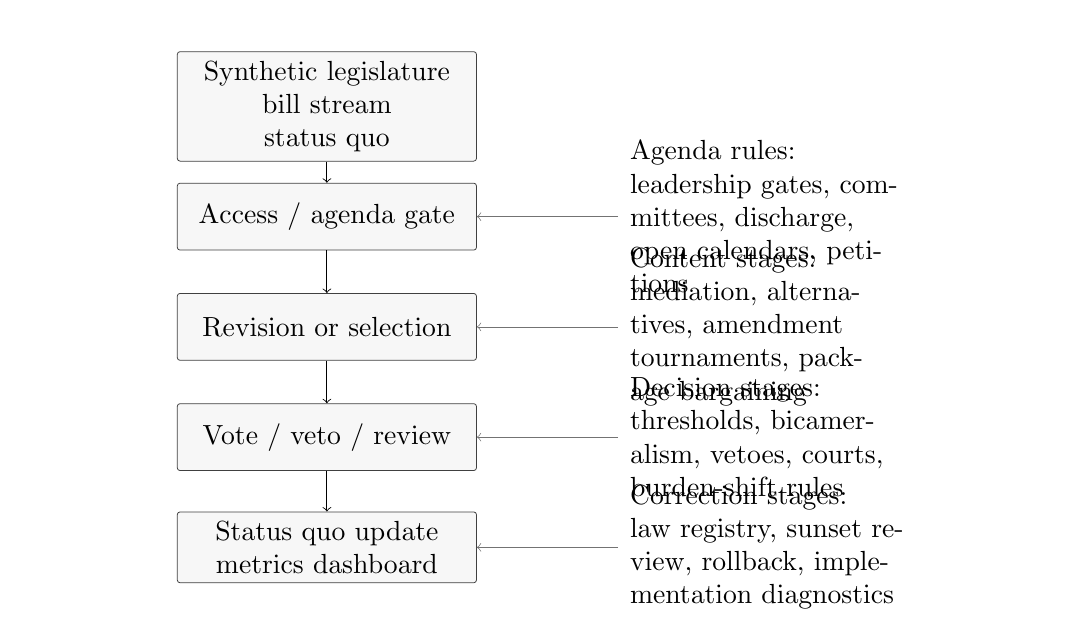
\begin{tikzpicture}[x=1mm,y=1mm]
\path[use as bounding box] (0,0) rectangle (130,74);
\tikzstyle{stage}=[draw=black!75, rounded corners=1pt, line width=0.28pt, align=center, minimum width=38mm, minimum height=8.5mm, fill=black!3]
\tikzstyle{side}=[align=left, text width=35mm]

\node[stage] (world) at (38,64) {Synthetic legislature\\bill stream\\status quo};
\node[stage] (access) at (38,50) {Access / agenda gate};
\node[stage] (revision) at (38,36) {Revision or selection};
\node[stage] (vote) at (38,22) {Vote / veto / review};
\node[stage] (metrics) at (38,8) {Status quo update\\metrics dashboard};

\draw[->, line width=0.3pt] (world) -- (access);
\draw[->, line width=0.3pt] (access) -- (revision);
\draw[->, line width=0.3pt] (revision) -- (vote);
\draw[->, line width=0.3pt] (vote) -- (metrics);

\node[side] at (94,50) {Agenda rules:\\leadership gates, committees, discharge, open calendars, petitions};
\draw[->, black!55, line width=0.25pt] (75,50) -- (access.east);

\node[side] at (94,36) {Content stages:\\mediation, alternatives, amendment tournaments, package bargaining};
\draw[->, black!55, line width=0.25pt] (75,36) -- (revision.east);

\node[side] at (94,22) {Decision stages:\\thresholds, bicameralism, vetoes, courts, burden-shift rules};
\draw[->, black!55, line width=0.25pt] (75,22) -- (vote.east);

\node[side] at (94,8) {Correction stages:\\law registry, sunset review, rollback, implementation diagnostics};
\draw[->, black!55, line width=0.25pt] (75,8) -- (metrics.east);
\end{tikzpicture}
\endgroup

